\documentclass[]{jeanmicheldoc}

\usepackage[hyphens]{url}
\usepackage[colorlinks=true]{hyperref}
\usepackage{tikz}
\usetikzlibrary{positioning}

\title{JeanMichel Document template}
\author{Mathieu Carrié}
\date{\today}
\institution{Blablabla}

\begin{document}

\maketitle

\newpage

\vspace{5cm}
\begin{abstract}
    blablablablablabla
\end{abstract}

\newpage

\section*{Unreferenced section}

blablabla

\newpage

\pagestyle{fancy}

{
    \hypersetup{linkcolor=blue!30!black}
    \tableofcontents
}

\newpage

\section{Introduction}
\section{Part 1}
    \subsection{Subsection 1}
    Gnagnagna
    \subsection{Subsection 2}
    Plop plop plop plop
\begin{itemize}
	\item \textbf{Prout}: Il a pas dit bonjour
    \item \textbf{Du coup}: ...
\end{itemize}

\section{Some figures}
    \begin{figure}[h!]
        \centering
        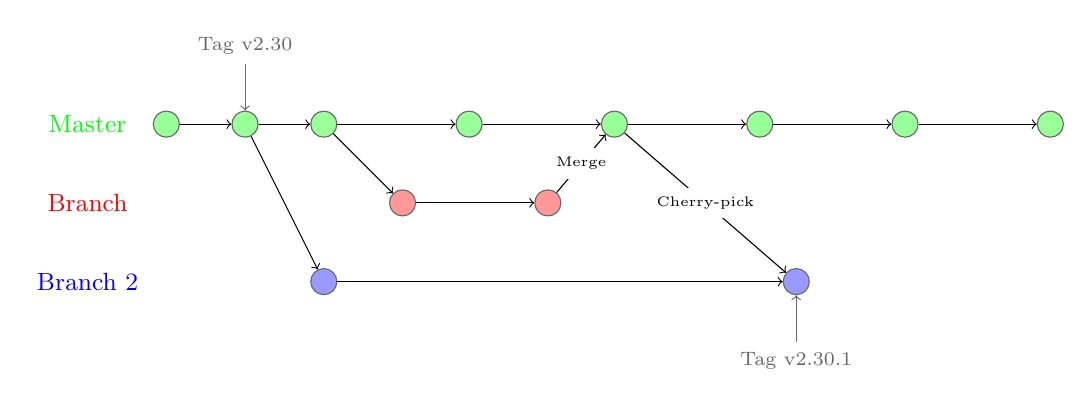
\begin{tikzpicture}
            \tikzstyle{label}   = [text=orange]
            \tikzstyle{tag}     = [text=black!60]
            \tikzstyle{tagline} = [draw=black!60]
            \tikzstyle{master}  = [circle, fill=green!40, draw=black!60]
            \tikzstyle{release} = [circle, fill=blue!40, draw=black!60]
            \tikzstyle{feature} = [circle, fill=orange!40, draw=black!60]
            \tikzstyle{hotfix}  = [circle, fill=red!40, draw=black!60]

            \node[label, text=green] (master) at (0,0) { \small Master };
            \node[label, text=red, below of=master] (hotfix) { \small Branch };
            \node[label, text=blue, below of=hotfix] (release) { \small Branch 2};

            \node[master, right of=master] (master1) {};
            \node[master, right of=master1] (master2) {};
            \node[master, right of=master2] (master3) {};
            \node[master, right=1.5 of master3] (master4) {};
            \node[master, right=1.5 of master4] (master5) {};
            \node[master, right=1.5 of master5] (master6) {};
            \node[master, right=1.5 of master6] (master7) {};
            \node[master, right=1.5 of master7] (master8) {};

            \draw[->] (master1) -- (master2);
            \draw[->] (master2) -- (master3);
            \draw[->] (master3) -- (master4);
            \draw[->] (master4) -- (master5);
            \draw[->] (master5) -- (master6);
            \draw[->] (master6) -- (master7);
            \draw[->] (master7) -- (master8);

            \node[release] (release1) at (3,-2) {};
            \node[release] (release2) at (9,-2) {};

            \draw[->] (master2) -- (release1);
            \draw[->] (release1) -- (release2);
            \draw[->] (master5) -- (release2) node[midway, fill=white]{\tiny Cherry-pick};

            \node[hotfix] (hotfix1) at (4, -1) {};
            \node[hotfix, right=1.5 of hotfix1] (hotfix2) {};

            \draw[->] (master3) -- (hotfix1);
            \draw[->] (hotfix1) -- (hotfix2);
            \draw[->] (hotfix2) -- (master5) node[midway, fill=white]{\tiny Merge};

            % Tags
            \node[tag, above of=master2] (tag1) {\scriptsize Tag v2.30};
            \draw[tagline, ->] (tag1) -- (master2);

            \node[tag, below of=release2] (tag2) {\scriptsize Tag v2.30.1};
            \draw[tagline, ->] (tag2) -- (release2);
        \end{tikzpicture}
        \caption{Caption}
        \label{fig:hotfix}
    \end{figure}

\section{Conclusion}

Use as a normal article class...

\end{document}
